\documentclass{beamer}

% Thème personnalisé
\usetheme{lines}

% Quelques importations pratiques
\usepackage{ifthen}      % pour des confitions dans les commandes
\usepackage{multicol}    % environnement multi colonnes
\usepackage{booktabs}    % pour des tables propres et sans colonnes
\usepackage{pifont}      % des symboles en plus
\usepackage{fontawesome} % utilisation de police d'icônes web

% Les variables générales proposées par Beamer
\title{Projet d'option informatique}
\subtitle{Deep Learning, traitement de langues naturelles et text mining}
\author{Damien \textsc{Douteaux} -- Vincent \textsc{Hocquemiller} -- Louis \textsc{Redonnet}}
\date{Jeudi 16 février 2017}

% Des commandes ponctuelles pour la présentation
\newcommand{\plus}{\textcolor{vertforet}{\faPlus{}}}
\newcommand{\moins}{\textcolor{bordeau}{\faMinus{}}}
\newcommand{\neutral}{\textcolor{bluenight}{\ding{70}}}

% Contenu de la présentation
% Le choix est ici de séparer chaque section dans un fichier contenu
% dans le répertoire text/. Cela permet d'y voir plus clair et de s'y
% retrouver plus vite dans le document
\begin{document}

% Slide de titre
\begin{frame}[plain]
	\titlepage
\end{frame}

% Sommaire
\section{Sommaire}
\begin{frame}
	\frametitle{Sommaire}
	\tableofcontents
\end{frame}

% Détails sur l'état de l'art
\section{Projets envisagés}
\subsection{Reconnaissance d'auteur}
\begin{frame}
	\frametitle{Auteur}
	\framesubtitle{Présentation du sujet}
	\paraTitle{Thème principal}
		\begin{itemize}
			\item Reconnaître l'auteur d'un texte
			\item Estimer le genre d'un auteur
		\end{itemize}
	
	\paraTitle{Plus-value possible}
		\begin{itemize}
			\item Peu (pas?) d'essais en Deep Learning.
			\item Peu d'essais en français.
		\end{itemize}

	\paraTitle{Applications possibles}
		\begin{itemize}
			\item Vérification de classification
			\item Analyse d'identité
			\item Validation auteur (cf. plagiat et/ou similarité)
		\end{itemize}
\end{frame}

\begin{frame}
	\frametitle{Auteur}
	\framesubtitle{Aspects techniques}
	\paraTitle{Bases de données}

		Extraitre de petites entités (paragraphes, tweets,...) via :
		\begin{itemize}
			\itemperso{Livres}Projet Gutenberg, Wikibooks,...
			\itemperso{Twitter}Récupération par API.
		\end{itemize}

	\paraTitle{Complexité}
		\begin{itemize}
			\item Problème ouvert
			\item Peu de sources		
		\end{itemize}
\end{frame}


\subsection{Inférence}
\begin{frame}
	\frametitle{Inférence}
	\framesubtitle{Présentation du sujet}
	\paraTitle{Thème principal}

		Extraire des relations entre phrases.
	
	\paraTitle{Plus-value possible}
		\begin{itemize}
			\item Peu d'essais en français.
			\item Comparaison entre langues.
		\end{itemize}

	\paraTitle{Applications possibles}
		\begin{itemize}
			\item Mise en avant de contradiction.
			\item Comparaison d'informations
		\end{itemize}
\end{frame}

\begin{frame}
	\frametitle{Inférence}
	\framesubtitle{Aspect technique}
	\paraTitle{Bases de données}
		\begin{itemize}
			\item Réutilisation de romans
			\item Articles de presse
			\item Stanford Natural Language Inference Corpus
		\end{itemize}

	\paraTitle{Complexité}
		\begin{itemize}
			\item Dépend de l'axe retenu
			\item Modélisation
			\item Grande variété de possibilités.
		\end{itemize}
\end{frame}

\subsection{Questions et réponses}
\begin{frame}
	\frametitle{Q\&A}
	\framesubtitle{Présentation du sujet}
	\paraTitle{Thème principal}
	
	Réponses automatiques à des questions simples.
	
	\paraTitle{Plus-value possible}
		\begin{itemize}
			\item Poursuivre les travaux en apprentissage par renforcement
		\end{itemize}

	\paraTitle{Applications possibles}
		\begin{itemize}
			\item Chatbox
			\item Proposition de services
		\end{itemize}
\end{frame}

\begin{frame}
	\frametitle{Q\&A}
	\framesubtitle{Aspects techniques}
	\paraTitle{Bases de données}
		\begin{itemize}
			\item Dialogues de films
			\item Autres difficiles à trouver (Facebook,...)
		\end{itemize}

	\paraTitle{Complexité}
		\begin{itemize}
			\item Utilisation de LSTM (technologie mature)
			\item Difficulté à trouver des BDDs 
			\item Difficulté de modélisation
			\item Manque de métrique pour évaluer
		\end{itemize}
\end{frame}

\subsection{Traduction}
\begin{frame}
	\frametitle{Traduction}
	\framesubtitle{Présentation du sujet}
	\paraTitle{Thème principal}

		Traduction à l'échelle d'un phrase par Deep Learning.
	
	\paraTitle{Plus-value possible}
		\begin{itemize}
			\item Un même réseau pour plusieurs langues.
			\item Trouver un autre cas d'usage?
		\end{itemize}
	
	\paraTitle{Applications possibles}

		Amélioration de résultats en traduction.
\end{frame}

\begin{frame}
	\frametitle{Traduction}
	\framesubtitle{Aspects techniques}
	\paraTitle{Bases de données}
	
		Tout ce qui est traduisible en plusieurs langues sur le web (cf. Linguee) :
		\begin{multicols}{2}
			\begin{itemize}
				\item Textes UE
				\item Brevets
				\item Documents légaux
				\item Site traduit
			\end{itemize}
		\end{multicols}

	\vspace*{-.2cm}

	\paraTitle{Complexité}
		\begin{itemize}
			\item Dépend de la précision
			\item Données présentes et technologies (LSTM) matures
		\end{itemize}
\end{frame}

\subsection{Analyse de sentiments}
\begin{frame}
	\frametitle{Sentiments}
	\framesubtitle{Présentation du sujet}
	\paraTitle{Thème principal}
		\begin{itemize}
			\item Classifier des phrases par sentiment.
			\item Prédire un sentiment (binaire ou avec une échelle).
		\end{itemize}

	\paraTitle{Plus-value possible}
		\begin{itemize}
			\item Combiner plusieurs approches.
			\item Problématique \og originale\fg.
		\end{itemize}

	\paraTitle{Applications possibles}
		\begin{itemize}
			\item Prendre le pouls de la \textit{twittosphère}.
			\item Classification de mails (injurieux ou non).
		\end{itemize}
\end{frame}

\begin{frame}
	\frametitle{Sentiments}
	\framesubtitle{Exemple d'arbre syntaxique}
	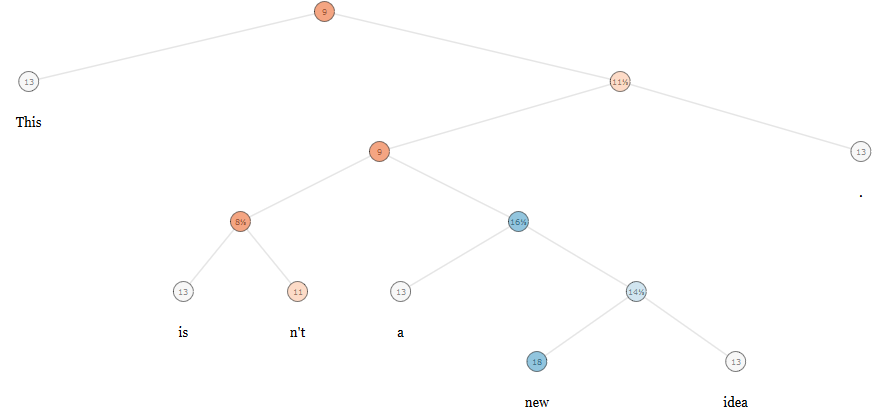
\includegraphics[width=\textwidth]{images/presentation/sampletree}
\end{frame}

\begin{frame}
	\frametitle{Sentiments}
	\framesubtitle{Aspects techniques}
	\paraTitle{Bases de données}
		\begin{itemize}
			\itemperso{IMDB, Amazon,...}Retours critiques de clients.
			\itemperso{Arbres syntaxiques}Stanford, 10000 arbres mais difficile à étendre (Amazon Turk).
		\end{itemize}

	\paraTitle{Complexité}
		\begin{itemize}
			\item Dépend de la précision et des outils.
			\item Base de données à aggréger.
			\item Grande variété de possibilités.
		\end{itemize}		
\end{frame}

% Explication du choix du sujet
\section{Choix du sujet}
\begin{frame}
	\frametitle{Comparaison des sujets}
	\begin{table}[ht]
		\centering
		\begin{tabular}{cccc}
			\toprule
			\textbf{Sujet} & \textbf{Plus-value} & \textbf{BDD} & \textbf{Complexité} \\
			\midrule
			\rule{0pt}{13pt}\textit{Auteur} & \neutral & \plus & \neutral \\
			\rule{0pt}{13pt}\textit{Inférence} & \neutral & \plus & \moins \\
			\rule{0pt}{13pt}\textit{Q\&A} & \neutral & \neutral & \moins \\
			\rule{0pt}{13pt}\textit{Traduction} & \moins & \plus & \moins \\
			\rule{0pt}{13pt}\textit{Sentiments} & \plus & \plus & \neutral \\
			\bottomrule
		\end{tabular}
	\end{table}

	\begin{center}
		\textbf{On retient le sujet d'analyse de sentiments.}
	\end{center}
\end{frame}

% Explications sur les bases de données
\section{Base de données}
\begin{frame}
	\frametitle{Prise de contact PAr}
	Récupération de diverses bases de données :
	\begin{itemize}
		\item Des contes de fée
		\item Des conversations de films
		\item Du texte de Wikipédia
		\item Des liens vers des BDDs
	\end{itemize}
	\begin{center}
		\textbf{Des bases intéressantes, mais peu liées à nos objectifs.}
	\end{center}
\end{frame}

\begin{frame}
	\frametitle{Des bases de données d'avis}
	\fontsize{9pt}{9pt}\selectfont
	\begin{table}[ht]
		\centering
		\begin{tabular}{cp{2.8cm}ccc}
			\toprule
			&\textbf{Nom} & \textbf{Type} & \textbf{Quantité} & \textbf{Origine} \\
			\midrule
			\textcolor{bordeau}{\faFilm} & \textit{Large Movie Review Dataset} & \textcolor{bordeau}{Cinéma} & $25 000\times2$ & Stanford \\
			&&& \\
			\textcolor{bordeau}{\faFilm} & \textit{Rotten Tomatoes Dataset} & \textcolor{bordeau}{Cinéma} & $1,6$Mb & Kaggle \\
			&&& \\
			\textcolor{bluenight}{\faTwitter} & \textit{Twitter Sentiment Corpus} & \textcolor{bluenight}{Tweets} & $5500$ & Niek Sanders \\
			&&& \\
			\textcolor{bluenight}{\faTwitter} & \textit{Twitter Sentiment Analysis Corpus} & \textcolor{bluenight}{Tweets} & $1 578 627$ & ? \\
			&&& \\
			\textcolor{vertforet}{\faCommentsO} & \textit{Sentiment Analyses Dataset} & \textcolor{vertforet}{Divers} & $9 645$ & Stanford \\
			&&& \\
			\textcolor{vertforet}{\faCommentsO} & \textit{UMICH S1650} & \textcolor{vertforet}{Blogs} & $40 000$ & Kaggle \\
			\bottomrule
		\end{tabular}
	\end{table}
	\begin{center}
		\textbf{Nécessité d'agglomérer les bases entre elles.}
	\end{center}
\end{frame}

% Premières réflexions sur les réseaux de neurones
\section{Réseau}
\begin{frame}
	\frametitle{Premières réflexions}
	\begin{itemize}
		\setlength{\itemsep}{1.2\baselineskip}
		\item Utilisation de \texttt{tensorflow}
		\item Peu de pistes sur l'architecture
		\item Calcul sur les serveurs du LIRIS
	\end{itemize}
\end{frame}

% Retours sur la gestion de projet
\section{Gestion de projet}
\begin{frame}
	\frametitle{Une semaine de décallage}
	\hfill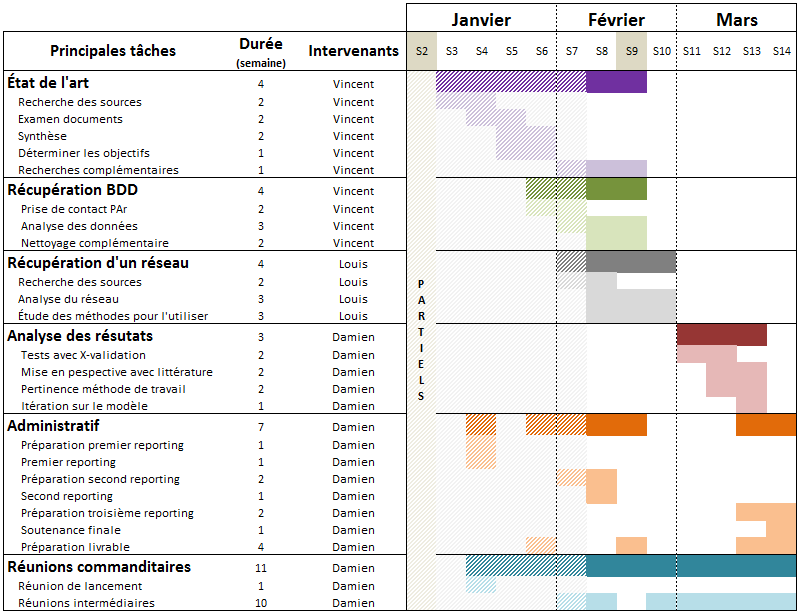
\includegraphics[width=.95\textwidth]{images/presentation/gantt}\hfill\rule{0pt}{0pt}
\end{frame}

% Conclusion du rapport
\section{Conclusion}
\nnsection{Conclusion}

%%% Local Variables:
%%% mode: latex
%%% TeX-master: "../../Rapport_dreches"
%%% End:


\end{document}